\documentclass[class=article, crop=false, 12pt]{standalone}
\usepackage[subpreambles=true]{standalone}
\usepackage{../.common/common}


\author{Tony Shing}
%\pretitle{Supplementary}

\topic{Note 1 (Math for Physics)}
\title{Single Variable Calculus on Mechanics}

\version{2025} % leave blank for omitting

\begin{document}

\maketitle

%\heading{Lecture}{Tony}

\begin{overview}
    \begin{itemize}
        \item Review on limits, differentiation and integration formulas. 
        \item Calculus relations between quantities in mechanics.
    \end{itemize}
\end{overview}


% content begins here
% Section %%%%%%%%%%%%%%%%%%%%%%%%%%%%%%%%%%%%%%%%%%%%%%%%%%%%
\section{Review on Calculus}

%%%%%%%%%%%%%%%%%%%
\subsection{Limits}
The naive definition of limit writes as:

\aleq{
    \lim_{x \to a} f(x) = L \quad (\text{where }L\neq \pm \infty)
}

which implies $f(x)$ is getting closer to $L$ when $x$ is getting closer to $a$.


%%%%%%%%%%%%%%%%%%%
\subsubsection{Two Sides Limits}

$x$ can approach $a$ from either the $+x$ or $-x$ direction. 
Therefore there can be two different limits.

\begin{itemize}
    \item \underline{Left hand limit}\ : $\displaystyle \lim_{x\to a^\red{-}} f(x) = L$
    \item \underline{Right hand limit} : $\displaystyle \lim_{x\to a^\red{+}} f(x) = L$
\end{itemize}

\bf{By definition}, we say $f(x)$ has a limit at $a$ only if \bf{both side limits at $a$ exist and equal}.

\begin{figure}
    \begin{subfigure}{0.33\textwidth}
        \centering
        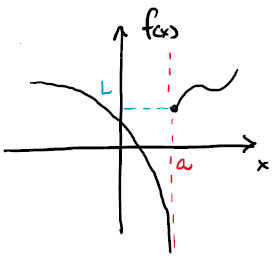
\includegraphics[height=10em]{lim1}
        \caption{\centering  L.H. limit $\to -\infty$ \\ R.H. limit $=L$ \\$\therefore$ Limit not exists at $a$}
    \end{subfigure}
    %
    \begin{subfigure}{0.33\textwidth}
        \centering
        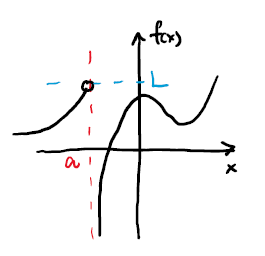
\includegraphics[height=10em]{lim2}
        \caption{\centering  L.H. limit $=L$ \\ R.H. limit $\to -\infty$ \\ $\therefore$ Limit not exists at $a$}
    \end{subfigure}
    %
    \begin{subfigure}{0.33\textwidth}
        \centering
        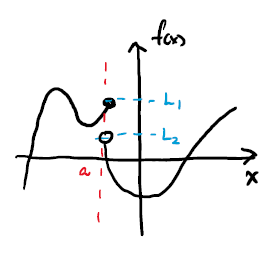
\includegraphics[height=10em]{lim3}
        \caption{\centering L.H. limit $=L_1$ \\ R.H. limit $=L_2$ \\ $\therefore$ Limit not exists at $a$}
    \end{subfigure}
\end{figure}

%%%%%%%%%%%%%%%%%%%
\subsubsection{Evaluation on Limits}

These formula are useful for resolving the limits of more complicated functions.
\blue{They work only if both the limits of $f(x)$ and $g(x)$ exist.}

\begin{itemize}
    \item \ul{Addition/Subtraction} : $\displaystyle \lim_{x\to a} [f(x) \pm g(x)] = \lim_{x\to a}f(x) \pm \lim_{x\to a} g(x)$
    
    \item \ul{Product} : $\displaystyle \lim_{x\to a} [f(x) \cdot g(x)] = (\lim_{x\to a} f(x))\cdot (\lim_{x\to a} g(x))$
    
    \item \ul{Quotient} : $\displaystyle \lim_{x\to a} \qty[\frac{f(x)}{g(x)}] = \frac{\displaystyle\lim_{x\to a}f(x)}{\displaystyle\lim_{x\to a} g(x)}$ \quad \blue{(require $\displaystyle \lim_{x\to a} g(x) \neq 0$)}
    
    \item \ul{Trigonometric} relation :
    $
        \begin{cases}
            \displaystyle \lim_{x\to \red{0}} \frac{\sin{x}}{x} = 1 \\
            \displaystyle \lim_{x\to \red{0}} \cos{x} = 1
        \end{cases}
    $
    
    \item \ul{Definition of natural exponential function} : $\displaystyle \lim_\red{n\to +\infty} \qty(1+\frac{x}{n})^n = e^x$
\end{itemize}

\bf{Note:} The formulas may look trivial, 
but they do require rigorous proofs to show that they work on all kinds of functions, 
which is a topic belonging to \it{mathematical analysis}.


%%%%%%%%%%%%%%%%%%%
\subsection{Differentiation}

The definition of differentiation on a function $f(x)$ is exactly evaluating the following limit:

\aleq{
    \lim_{\Delta x \to 0} \frac{f(x+\Delta x) - f(x)}{\Delta x} \ \defeq\  \dv{x} f(x) \ \text{ or }\  f'(x)
}
(Both notation $\dv{x}$ and $f'(x)$ are commonly used, but I will stick to $\dv{x}$ for better readability.)\\ 

Geometrically, differentiation means evaluating the slope of (tangent lines of) the function.

\begin{center}
    \begin{minipage}{0.3\textwidth}
        \centering
        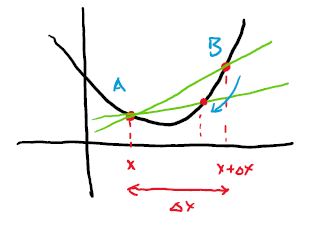
\includegraphics[width=\textwidth]{secant}
    \end{minipage}
    %
    \hspace{0.05\textwidth}
    %
    \begin{minipage}{0.5\textwidth}
        \centering
        \red{
            Slope of line $\overline{AB}  = \dfrac{f(x+\Delta x) - f(x)}{\Delta x}$ \\[1em]
            When $\Delta x \to 0$, $\overline{AB}$ become a tangent line at $x$.
        }
    \end{minipage}
\end{center}


%%%%%%%%%%%%%%%%%%%
\subsubsection{Evaluation of Differentiation}

These formula are important for evalutaing differentiation of more complicated functions.
\blue{They work only if both the differentiation of $f(x)$ and $g(x)$ exist.}

\begin{itemize}
    \item \ul{Addition/Subtraction} : $\dvv{x}[f(x)\pm g(x)] = \dvv{x}f(x) \pm \dvv{x}g(x)$
    
    \item \ul{Scaling} : $\dvv{x}[kf(x)] = k\dvv{x}f(x)\qquad (\text{given }k = \text{ constant})$

    \item \ul{Product rule} : $\dvv{x}[f(x)\cdot g(x)] = \qty[\dvv{x}f(x)]\cdot g(x) + f(x)\cdot \qty[\dvv{x} g(x)]$
    
    \item \ul{Quotient rule} : $\dvv{x}\qty[\frac{f(x)}{g(x)}] = \dinv{[g(x)]^2}\qty[g(x)\cdot \dvv{x}f(x) - f(x)\cdot \dvv{x}g(x)]$ \\[1em]
        (Note that quotient rule is the same as applying product rule on $\displaystyle \dvv{x}\qty[f(x)\cdot \inv{g(x)}]$)
    
    \item \ul{Chain rule} : $\dvv{x}[g(f(x))] = \dvv{[f(x)]}g(f(x)) \cdot \dvv{x}f(x)$
\end{itemize}

\begin{minipage}{0.6\textwidth}
    \begin{itemize}
    \item \ul{Inverse function} : $\dvv{x} f^{-1}(x) = \dinv{\eval{\dvv{y}f(y)}_{y=f^{-1}(x)}}$
        
    
    \item \ul{Polynomial function} : $\dvv{x} x^n = nx^{n-1}$
    

    \end{itemize}
\end{minipage}
%
\begin{minipage}{0.4\textwidth}
    \centering
    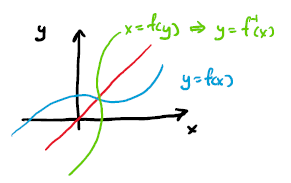
\includegraphics[width=0.8\textwidth]{inv_func}
    \\
    \scriptsize Inverse function = Diagonal flip
\end{minipage}


\begin{itemize}
        \item \ul{Trigonometric function} : $\dvv{x} 
        \begin{cases} \sin{x}\\ \cos{x}\\ \tan{x} \end{cases}
        =\;
        \begin{cases} \cos{x}\\ -\sin{x}\\ \sec^2{x} \end{cases}
        $

    \item \ul{Exponential function} : $\dvv{x} 
        \begin{cases} e^{x}\\ \ln{x} \end{cases}
        =\;
        \begin{cases} e^{x}\\ \dinv{x} \end{cases}
        $
\end{itemize}


%%%%%%%%%%%%%%%%%%%
\subsection{Integration}

\subsubsection{Definite Integral (Riemann Integral)}

The geometrical meaning to definite integral is to compute the area under curve. 
The construction is through the following steps:

\begin{figure}[h]
    \centering
    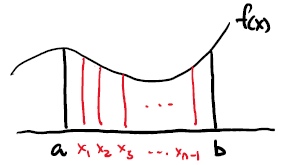
\includegraphics[width=0.3\textwidth]{int_slice}
\end{figure}


\begin{enumerate}
    \item Choose $n-1$ points between $[a,b]$:
    \aleq{
        a \,\red{<x_1 < x_2 < ... <x_{n-1} <} \,b = \blue{\substack{\scriptstyle \text{separate into }\\ \text{total }n\text{ steps}}}
    }

    \item Within each strip, pick an arbitrary point \blue{$x=\xi_i$} at its base. 
    The strip's height can be approximated as $\approx f(\blue{\xi_i})$.

    \begin{center}
        \begin{minipage}{0.3\textwidth}
            \centering
            \begin{figure}[h]
                \centering
                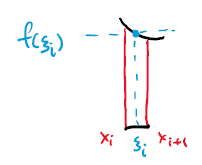
\includegraphics[width=0.6\textwidth]{int_strip}
            \end{figure}
        \end{minipage}
        %
        $\quad \Rightarrow \quad$
        %
        \begin{minipage}{0.3\textwidth}
            \centering
            \begin{figure}[h]
                \centering
                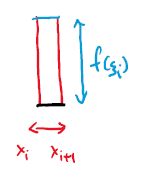
\includegraphics[width=0.4\textwidth]{int_strip2}
            \end{figure}
        \end{minipage}
    \end{center}
    

    \item The approximated area of each strip is then (height)$\times$(base) $\approx f(\blue{\xi_i})\times [\red{x_{i+1}-x_i}]$.\\
        $\Rightarrow$ Total area under curve = Summing the areas of all strips 
        \aleq{
            =\sum_{i=0}^{n-1} f(\blue{\xi_i})\cdot [\red{x_{i+1}-x_i}] \qquad \green{(\text{with }x_0 = a, x_n = b)}
        }

    \item Finally take the width of each strip $[\red{x_{i+1}-x_i}] = \red{\Delta x_i}$ limit to $0$. \\
        \blue{No matter how "arbitrary" we chose $\xi_i$ within $[x_i, x_{i+1}]$, 
        the width become so small so that the height of the strip is limit to $f(\xi_i)$.}
        
\end{enumerate}

$\Rightarrow$ Area under curve $\approx$ Summing the area of infinitely many strips that have widths $\approx 0$. 
Here comes the formal definition:

\aleq{
    \int_b^a f(\blue{x}) \red{\dd{x}} \; \defeq\;  \lim_{\Delta x_i \to 0}\, \sum_{i=0}^{n-1} f(\blue{\xi_i})\red{\Delta x_i}
}


%%%%%%%%%%%%%%%%%%%
\subsubsection{An alternative interpretion of definite integral}

Other than the area under curve, we can also interpret a definite integral as a weighted sum. This is in fact more useful in physics' applications.

\begin{minipage}{0.7\textwidth}
    \begin{itemize}
        \item \ul{\nth{1} intepretation - Area under curve}
            \aleq{
                \int_b^a f(\blue{x}) \red{\dd{x}} \; 
                \defeq\;  
                \lim_{\Delta x_i \to 0}\, \tkn{s1}{\cul[green]{\sum_{i=0}^{n-1}}}\enspace 
                \tkn{h1}{\cul[blue]{f(\blue{\xi_i})}}\cdot
                \tkn{w1}{\cul[red]{\red{\Delta x_i}}}
            }
            \addArrow[green]{s1}{(0,-4.5ex)}{$\substack{\text{Sum} \\ \text{them all}}$}
            {(0,-4ex)}
            \addArrow[blue]{h1}{(0,-4ex)}{$\substack{\text{height of} \\ \text{strips}}$}
            {(0,-1.5ex)}{(0,-0.5ex)}
            \addArrow[red]{w1}{(2ex,-4ex)}{$\substack{\text{width of} \\ \text{strips}}$}
            {(0,-1.5ex)}{(0,-0.5ex)}
        \\
    \end{itemize}
\end{minipage}
\begin{minipage}{0.3\textwidth}
    \hfill \\[1.5em]
    \centering
    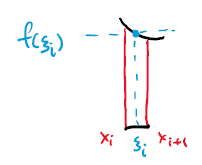
\includegraphics[width=0.6\textwidth]{int_strip}
    \\
    \scriptsize \hspace{5ex} Interpret as sum of area 
\end{minipage}


\begin{minipage}{0.7\textwidth}
    \begin{itemize}
        \item \ul{\nth{2} intepretation - Weighted sum}
            \aleq{
                \int_b^a f(\blue{x}) \red{\dd{x}} \; 
                \defeq\;  
                \lim_{\Delta x_i \to 0}\, \tkn{s2}{\cul[green]{\sum_{i=0}^{n-1}}}\enspace 
                \tkn{h2}{\cul[blue]{f(\blue{\xi_i})}} \cdot
                \tkn{w2}{\cul[red]{\red{\Delta x_i}}}
            }
            \addArrow[green]{s2}{(-5.5ex,-3.5ex)}{$\substack{\text{Sum} \\ \text{them all}}$}
            {(0,-4ex)}
            \addArrow[blue]{h2}{(0,-4ex)}{$\substack{\text{"weight"}\\\text{assigned to the} \\ \text{interval } [x_i, x_{i+1}]}$}
            {(0,-1.5ex)}{(0,-1.5ex)}
            \addArrow[red]{w2}{(5ex,-4ex)}{$\substack{\text{length of} \\ \text{interval } \\ [x_i, x_{i+1}]}$}
            {(0,-1.5ex)}{(0,-1.5ex)}
        \\
    \end{itemize}
\end{minipage}
\begin{minipage}{0.3\textwidth}
    \hfill \\[1.5em]
    \centering
    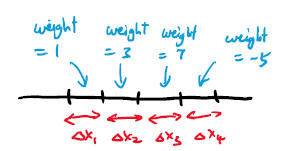
\includegraphics[trim=-6ex 0 0 0, width=0.9\textwidth]{int_weight}
    \\
    \scriptsize \hspace{5ex} Interpret as weighted sum 
\end{minipage}

\vspace{2em}


\begin{example} Distribution graph of students' heights\\

    Suppose a class of 20 students have the following heights (in cm):

    \begin{center}
        165 165 166 167 167 167 168 168 169 169 169 169 170 170 172 172 172 173 174 174
    \end{center}

    Their total height is the the sum of each possible heights but weighted by number of people of that height:
    \aleq{
        \text{Total height} &= \sum \text{"weight"} \times \text{height} \\
        &= \sum_h \qty(\substack{\text{Number of students}\\\text{with height } h})\times \qty( \text{height }h) \\
        &= 2 \times 165 + 1 \times 166 + 3 \times 167 + 2 \times 168 + 4\times 169 \\
            &\quad + 2\times 170 + 3\times 172 + 1\times 173 + 2\times 174
    }

    If we plot out the bar chart, we can see the similarity to area under curve: \\ 
    (Total height of students) = (Sum of all bars' height) $\times 1$ = (Total area under every bar). 

    \begin{center}
        \begin{minipage}{0.45\textwidth}
            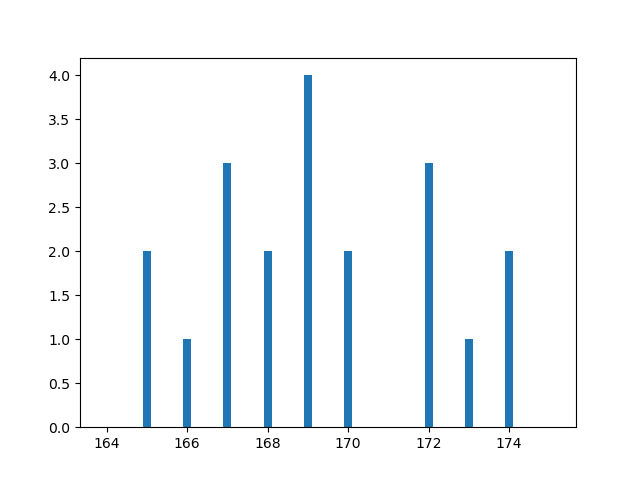
\includegraphics[width=\textwidth]{bar1}
        \end{minipage}
        %
        $\Rightarrow$
        %
        \begin{minipage}{0.45\textwidth}
            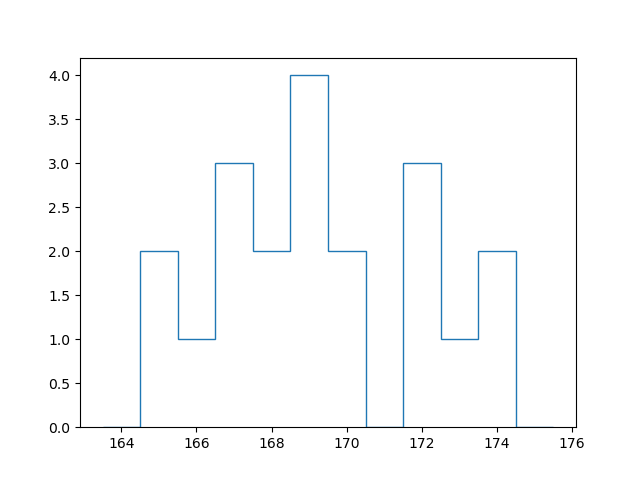
\includegraphics[width=\textwidth]{bar2}
        \end{minipage}
    \end{center}
    

\end{example}

Then we can transition from discrete to continuous distribution: 
\begin{itemize}
    \item \bf{A standalone number $\rightarrow$ An interval between two numbers.}\\
    E.g. A height of 163 cm $\rightarrow$ A range of height between $[162.5, 163.5] $cm

    \item \bf{Height of a bar $\rightarrow$ The area under the bar}\\
    E.g. Portion of students with height between the range $[162.5, 163.5] $cm
\end{itemize}

When the interval width is limit to $0$, the weighted sum arrives at the same definition as a definite integral. 


%%%%%%%%%%%%%%%%%%%
\subsubsection{Indefinite Integral}

In contrast to definite integral, the definition of indefinite integral is purely algebaric. Given a function $f(x)$, 

\begin{itemize}
    \item If there exists another function $F(x)$ such that $\dvv{x}F(x) = f(x)$,
    then $F(x)$ is called the \bf{antiderivative} or \bf{primitive} of $f(x)$.

    \item The \bf{indefinite integral} of $f(x)$ is the \bf{set of all antiderivative of $f(x)$}. 
    
\end{itemize}

The emphasis is on the term "set" because $f(x)$ always has infinitely many antiderivatives.
This is also the reason why a constant $C$ should always be added after computing indefinite integral.

\newpage
For example,
\aleq{
    f(x) &= x^2 \\
    \Rightarrow \int f(x) \dd{x} &= \frac{x^3}{3} \red{\ +\ C} \\
    &= \qty{\text{Set of all functions in the form }\frac{x^3}{3} + \text{ real number}}
}


%%%%%%%%%%%%%%%%%%%
\subsubsection{Evaluation of Indefinite Integral}

These formula are important for evalutaing integration of more complicated functions.
(Yet not every function can be integrated analytically.)
\blue{The proofs for these formula can be reached directly by reversing the differentiation operation.}

\begin{itemize}
    \item \ul{Addition/Subtration} : $\displaystyle \int f(x) \pm g(x) \dd{x} = \int f(x) \dd{x} \pm \int_a^b g(x) \dd{x}$
    
    \item \ul{Scaling} : $\displaystyle \int kf(x) \dd{x} = k \int f(x) \dd{x}\qquad (\text{given }k = \text{ constant})$

    \item \ul{Integration by Part} \red{(Corresponding to product rule)} :
    \aleq{
        \int f(x) \cdot \dvv{x}g(x) \dd{x} &= f(x)\cdot g(x) - \int \dvv{x} f(x) \cdot g(x) \dd{x} \\
        \green{f(x)\cdot g(x)}\ &\green{=} \green{\int f(x) \cdot \dvv{x}g(x) \dd{x} + \int \dvv{x} f(x) \cdot g(x) \dd{x}} \\
        \green{\Rightarrow\quad \dvv{x}(f(x)\cdot g(x))}\ &\green{=} \green{f(x) \cdot \dvv{x}g(x) + \dvv{x} f(x) \cdot g(x)}
    }

    \item \ul{Integration by Change of Variable} \red{(Corresponding to chain rule)} :
    \aleq{
        \int g[f(x)] \cdot \dvv{x}f(x) \dd{x} &= \int g[f(x)]\cdot \dd{[f(x)]} \\
        = \int g(u) \dd{u} \eval_{u=f(x)}
    }

    \item \ul{Polynomial function} : $\displaystyle \int x^n \dd{x} = \dfrac{x^{n+1}}{n+1} +C$ 
    
    \item \ul{Trigonometric function} : $\displaystyle \int
        \begin{cases} \sin{x}\\ \cos{x}\\ \sec^2{x} \end{cases} \dd{x}
        =\;
        \begin{cases} -\cos{x}\\ \sin{x}\\ \tan{x} \end{cases} +C
        $

    \item \ul{Exponential function} : $\displaystyle \int
        \begin{cases} e^{x}\\ \dinv{x} \end{cases} \dd{x}
        =\;
        \begin{cases} e^{x}\\ \ln{|x|} \end{cases}  +C
        $

    \item \ul{Substitution of trigonometric function}
    \aleq{
        \int \sqrt{r^2-x^2} \dd{x} &\Rightarrow \red{\text{ Subst. }x=r\sin\theta} 
        \Rightarrow \begin{cases} \sqrt{r^2-x^2} = r\cos\theta \\ \dd{x} = r\cos\theta\dd{\theta}\end{cases} \\
        \int \sqrt{r^2+x^2} \dd{x} &\Rightarrow \red{\text{ Subst. }x=r\tan\theta}
        \Rightarrow \begin{cases} \sqrt{r^2+x^2} = r\sec\theta \\ \dd{x} = r\sec^2\theta\dd{\theta}\end{cases} \\
        \int \sqrt{x^2-r^2} \dd{x} &\Rightarrow \red{\text{ Subst. }x=r\sec\theta}
        \Rightarrow \begin{cases} \sqrt{x^2-r^2} = r\tan\theta \\ \dd{x} = r\sec\theta\tan\theta\dd{\theta}\end{cases} \\
    }
\end{itemize}




%%%%%%%%%%%%%%%%%%%
\subsubsection{Fundamental Theorem of Calculus}

Up to this point, we are in fact looking at two different use cases of the symbol $\int$:

\begin{enumerate}
    \item $\int_a^b$ represents definite integral, which represents the area under curve between $[a,b]$.
    \aleq{
        \int_a^b \sim \lim_{\Delta x\to 0} \sum_{i=0}^{n-1}
    }
    Calculating this limit of sum looks quite tedious. 

    \item $\int$ represents indefinite integral, which is the opposite operation of differentiation.
    \aleq{
        \int f(x) \dd{x} = F(x) \quad\Leftrightarrow\quad \dvv{x} F(x) = f(x)
    }
    Simplification formulas are straightly derived from reversing differentiation.
\end{enumerate}

Of course, nowadays we know that the two's calculations are basically the same. 
(And that's why mathematicians assigned them the same symbol.) 
However, for rigourous mathematics needs, we need an extra step to show that they are intrinsically the same,
which is why we have the \bf{fundamental theorem of calculus}.


\begin{itemize}
    \item \ul{\nth{1} fundamental theorem of calculus} \red{(definite $\to$ indefinite)} : \\[1em]
    An antiderivative $F(x)$ can be constructed from a definite integral on $f$ over an interval with a varying upper bound, i.e.,
    \aleq{
        F(x) = \int^x_b f(t) \dd{t}
    }

    \item \ul{\nth{2} fundamental theorem of calculus} \red{(indefinite $\to$ definite)} : \\[1em]
    The definite integral on $f(x)$ over an interval can be computed by the subtraction between the antiderivatives $F$ at the bounds, i.e.,
    \aleq{
        \int_a^b f(x) \dd{x} = F(b) - F(a)
    }
\end{itemize}

The proofs can be found with clear explanation on wiki, so I shall omit them in this note.

\url{https://en.wikipedia.org/wiki/Fundamental_theorem_of_calculus#Formal_statements}




\linesep
% Section %%%%%%%%%%%%%%%%%%%%%%%%%%%%%%%%%%%%%%%%%%%%%%%%%%%%
\section{Calculus Relations in Mechanics}


%%%%%%%%%%%%%%%%%%%
\subsection{Relation between $s,v,a$}

In secondary school textbook, we have the definitions:

\begin{itemize}
    \item Displacement $s$ 
    \item Average velocity $v \sim  \dfrac{\Delta s}{\Delta t} = \dfrac{\text{Change in displacement}}{\text{time}}$
    \item Average acceleration $a \sim \dfrac{\Delta v}{\Delta t} = \dfrac{\text{Change in velocity}}{\text{time}}$
\end{itemize}

But the term "average" is never accurate to describe things.

\begin{center}
    \begin{minipage}{0.3\linewidth}
        \centering
        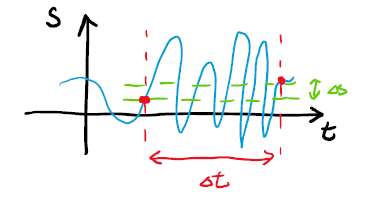
\includegraphics[width=\textwidth]{vary_s}
    \end{minipage}
    \hspace{0.05\textwidth}
    \begin{minipage}{0.4\linewidth}
        \centering
        \blue{
            Average velocity $\dfrac{\Delta s}{\Delta t}$ \\[1em]
            cannot describe drastic motion.
        }
    \end{minipage}
\end{center}


For accurate description, we need to shorten the time separation between two measurements as much as possible, i.e. limit to $0$.\\
$\Rightarrow$ Instantaneous quantities = quantity measured at a "single" time point.

\begin{itemize}
    \item Instantaneous velocity $= \displaystyle \lim_{\Delta t\to 0} \dfrac{\Delta s}{\Delta t} = \dvv{t}s(t)$
    \item Instantaneous acceleration $= \displaystyle \lim_{\Delta t \to 0} \dfrac{\Delta v}{\Delta t} = \dvv{t}v(t)$ 
\end{itemize}
\aleq{
    \Acboxed{
    s(t) \xrightleftharpoons[\int \dd{t}]{\hspace{0.5cm}\dv{t}\hspace{0.5cm}} v(t)
    \xrightleftharpoons[\int \dd{t}]{\hspace{0.5cm}\dv{t}\hspace{0.5cm}} a(t)
    }
}

\hfill\\
\begin{example} Constant Acceleration Motion\\

    By definition, the acceleration $a(t) = a$ is a constant. 
    Finding velocity and displacement are then straightforward integration.

    \begin{itemize}
        \item \ul{Velocity} : $v(t) = \displaystyle \int a \dd{t} = at + C_1$ \\[0.5em]
        At $t=0$, $v(0) = C_1 =$ initial velocity, which is usually denoted as $u$ in textbook.
        \aleq{
            \Rightarrow v(t) = v(0) + at
        }

        \item \ul{Displacement} : $s(t) = \displaystyle \int v(t) \dd{t} = v(0)t + \half at^2 + C_2$ \\[0.5em]
        At $t=0$, $s(0) = C_2 =$ initial displacement.
        \aleq{
            \Rightarrow s(t) = s(0) + v(0)t + \half at^2
        }
    \end{itemize}
    
    In fact, out of the 4 formulas we usually found in textbook, only 2 of them are independent.
    \aleq{
        \bcase{
            v(t) &= v(0) + at \tkm{suvat1}\\
            s(t) &= s(0) + v(0)t + \half at^2 \tkm{suvat2}\\ 
            s(t)-s(0) &= \dfrac{v(t)-v(0)}{2}t \tkm{suvat3}\\ 
            v(t)^2 - v(0)^2 &= 2a[s(t)-s(0)] \tkm{suvat4}
        }
    }
    \addArrow[red]{suvat1}{(20ex,-0.5ex)}
    {$\substack{\displaystyle\text{Definition}\\\displaystyle\text{nothing to explain}}$}
    {(1ex,0.5ex)}{(4ex,-1ex)}
    \addArrow[red]{suvat2}{(8ex,0.5ex)}{}{(1ex,0.5ex)}
    \addArrow[green]{suvat3}{(16ex,-0.5ex)}
    {$\substack{\displaystyle\text{Can be derived by}\\\displaystyle\text{substitution of the above 2}}$}
    {(1ex,0.5ex)}{(6ex,-1ex)}
    \addArrow[green]{suvat4}{(8ex,0.5ex)}{}{(1ex,0.5ex)}

    Having only 2 independent equations implies that we can at most solve 2 unknowns out of the 5 alphabets "SUVAT".
    So in such standard question, you should always able to find the info of at least 3 of the alphabets.
    Only then you can solve the remaining 2. 

\end{example}

%%%%%%%%%%%%%%%%%%%
\subsection{Force and Energy}

Work done is the fundamental relation between force and energy:
\aleq{
    \text{W.D.} = F \cdot \Delta s = \qty(\substack{\displaystyle\text{Average}\\\displaystyle\text{Force}})\cdot \qty(\text{Displacement})
}

For a time varying force $F(t)$, consider the W.D. in a very short time interval $[t_i, t_{i+1}]$
\aleq{
    \Delta\text{W.D.}_i &\approx \frac{F(t_i)+F(t_{i+1})}{2} \cdot [s(t_{i+1}) - s(t_i)] \\
    &= \frac{F(t_i)+F(t_{i+1})}{2} \cdot \qty[\frac{s(t_{i+1}) - s(t_i)}{\green{t_{i+1}-t_i}}](\green{t_{i+1}-t_i})
}

The the total W.D. in a long period time 
\aleq{
    &= \text{Sum of all W.D. of many small time interval}\\
    &= \sum_i \qty[\frac{F(t_i)+F(t_{i+1})}{2}] \cdot \qty[\frac{s(t_{i+1}) - s(t_i)}{t_{i+1}-t_i}](t_{i+1}-t_i)
}

Take limit to the time interval $\Delta t = t_{i+1}-t_i \to 0$, then $t_{i+1}\approx t_i$ and $F(t_{i+1})\approx F(t_i)$.
\addArrow[blue]{Fstar}{(18ex,3.5ex)}
{$\substack{\displaystyle\text{More commonly, force is provided} \\ \displaystyle\text{as a function of displacement}}$}
{(4ex,2ex)}{(12ex,-1ex)}
\aleq{
    \text{W.D} &\rightarrow \int \frac{F(t)+F(t)}{2} \cdot \qty[\dvv{s(t)}{t}] \dd{t}\\
    &= \int F(t)\cdot v(t) \dd{t} \\
    &= \int F(t) \cdot \dd{[s(t)]} \\
    &= \int \tkn{Fstar}{\cul[blue]{F^*[s(t)]}} \dd{[s(t)]}
}

\red{(Notice the sign difference)} If the force is associated with a potential energy,
the change in P.E. formula acquires a minus sign.
\aleq{
    \Acboxed{
        \text{W.D.}_{\red{(\text{by }F)}} = \int F(s) \dd{s}  \qquad\Leftrightarrow\qquad
        \text{Change in P.E.} = \tkn{PEminus}{\red{-}} \int F(s) \dd{s}
    }
}
\addArrow[red]{PEminus}{(0,-5ex)}
{$\substack{\displaystyle\text{W.D. \bf{by} a force due to potential} \Rightarrow \text{ loss in P.E.} \\ 
    \displaystyle\text{W.D. \bf{against} a force due to potential }\Rightarrow \text{ gain in P.E.}}$}
{(0,-0.5ex)}{(0,-1.5ex)}

\hfill\\[1em]
Finally, their relations to force is by differentiation.
\aleq{
    \Acboxed{
        F = \dvv{s}\qty(\text{W.D.}_{\red{(\text{by }F)}}) \qquad\Leftrightarrow \qquad
        F = \tkn{PEminus2}{\red{-}}\dvv{s}\text{(P.E.)}
    } 
}
\addArrow[red]{PEminus2}{(0,-5ex)}{Please remember the $-$ve\\as if it is a definition}
{(0,-0.5ex)}{(0,-1.5ex)}

\hfill\\
\begin{example} Gravitational force \& potential energy (PE)

    \aleq{
        F(\tkn{Fr}{\blue{r}}) = -\frac{GMm}{\blue{r}^2}
    }\\
    \addArrow[blue]{Fr}{(0,-3.5ex)}
    {Force is a function of distance from the masses}
    {(0,-1ex)}{(0,-0.5ex)}
    
    Then the W.D. by gravitational force from position $r_1$ to $r_2$ can be computed by integrating the force
    \aleq{
        \text{W.D.} &= \int_{r_1}^{r_2} -\frac{GMm}{r^2}\dd{r} \\
        &= \qty(\frac{GMm}{r_2}) - \qty(\frac{GMm}{r_1}) \\
        &= -\qty(-\frac{GMm}{r_2}) - \qty(-\frac{GMm}{r_1}) \\
        &= \tkn{GPEminus}{\red{-}}\qty(\text{GPE at }r_2 - \text{GPE at }r_1)
    }
    \addArrow[red]{GPEminus}{(0,-3ex)}
    {$\substack{\displaystyle\text{W.D. by gravitation } \Rightarrow \text{ loss in PE} \\ \displaystyle\text{W.D. against gravitation }\Rightarrow \text{ gain in PE}}$}
    {(0,-0.5ex)}{(0,-2ex)}

    \hfill\\[1em]
    Reversely, we take the \red{minus} differentiation to the PE formula to find the force due to gravitation.
    \aleq{
        \text{PE} &= -\frac{GMm}{r} \\
        \text{Gravitational force} &= \tkn{Fminus}{\red{-}} \dvv{r}(\text{PE}) = -\frac{GMm}{r^2}
    }\\
    \addArrow[red]{Fminus}{(0,-3.5ex)}{Negative sign indicates\\the force as attractive}
    {(0,-0.5ex)}{(0,-2ex)}

\end{example}

\newpage
%%%%%%%%%%%%%%%%%%%
\subsection{Momentum, Impulse and Newton \nth{2} Law}

Momentum and impulse is in fact an equivalent description to Newton's \nth{2} Law.

\begin{center}
    \begin{tabular}{ >{\centering\arraybackslash}m{15em} | >{\centering\arraybackslash}m{15em} }
        \ul{Force \& Acceleraton} & \ul{Impulse \& Momentum} \\ 
        $F=ma$ & $I=\Delta(mv)$ \\  
        Apply a force & Apply an impulse \\
        Get acceleration & Change in momentum    
    \end{tabular}
\end{center}


Recall that the definition of impulse as \\[-2.5em]
\begin{center}
    \begin{minipage}{0.5\textwidth}
        \aleq{
            I &\sim F\cdot \Delta t \\
            &= \qty(\text{Applied Force})\cdot \qty(\text{Duration}) \\
            &= \text{Area under curve in F-t graph} \\
            &= \text{Change in momentum}
        }
    \end{minipage}
    %
    \hspace{0.05\textwidth}
    %
    \begin{minipage}{0.35\textwidth}
        \centering
        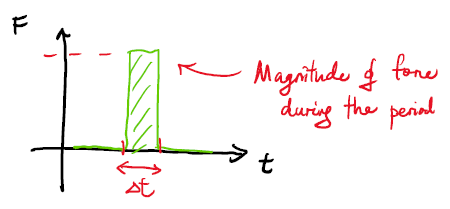
\includegraphics[width=\textwidth]{imp_naive}
    \end{minipage}
    \hfill
\end{center}

But in reality, when objects collide, the applied force is not constant during the whole time.
Imagine what should actually happen when you hit a baseball with a bat:


\begin{center}
    \begin{minipage}{0.4\linewidth}
        \centering
        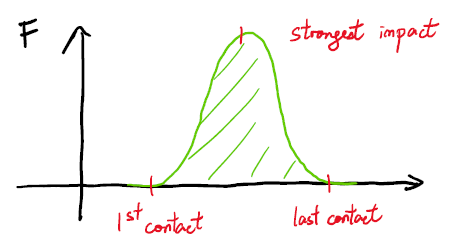
\includegraphics[width=\textwidth]{imp_real}
    \end{minipage}
    %
    \begin{minipage}{0.4\linewidth}
        \centering
        \green{\ul{This is the F-t graph in reality}}
    \end{minipage}
    \\[1em]
    %
    \begin{minipage}{0.3\linewidth}
        \centering
        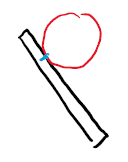
\includegraphics[height=8em]{hit1}\\
        \ul{First contact} \\
        Contact area $\sim 0$ \\
        $\Rightarrow F\sim 0$ 
    \end{minipage}
    %
    \begin{minipage}{0.3\linewidth}
        \centering
        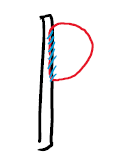
\includegraphics[height=8em]{hit2}
        \ul{Strongest impact} \\
        Contact area $=$ max \\
        $\Rightarrow F= $ max 
    \end{minipage}
    %
    \begin{minipage}{0.3\linewidth}
        \centering
        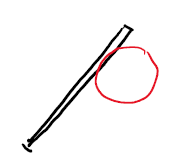
\includegraphics[height=8em]{hit3}
        \ul{Right before separate} \\
        Contact area $\sim 0$ \\
        $\Rightarrow F\sim 0$ 
    \end{minipage}
\end{center}

\hfill \\
\bf{In general, force should be taken as a function of time.} \\

Similar to how we computed W.D., 
we can first consider the change in momentum in a very short time interval $[t_i, t_{i+1}]$
\aleq{
    \Delta(mv)_i = I_i &\approx \frac{F(t_i)+F(t_{i+1})}{2} (t_{i+1} - t_i) \\
}

The the total change in momentum in a long period time 
\aleq{
    \sum_i \Delta(mv)_i = \sum_i I_i &= \text{Sum of all impulse of many small time interval}\\
    &= \sum_i \qty[\frac{F(t_i)+F(t_{i+1})}{2}] (t_{i+1}-t_i)
}

Take limit to the time interval $\Delta t = t_{i+1}-t_i \to 0$, then $t_{i+1}\approx t_i$ and $F(t_{i+1})\approx F(t_i)$.
\aleq{
    \int \dd{(mv)} = I &\rightarrow \int \frac{F(t)+F(t)}{2} \dd{t}\\
    &= \int F(t) \dd{t}
}

i.e. The "real" impulse-momentum relation should be reprensented with integral.
We can also differentiate both side by $t$ to recover momentum's relation with force . 
\aleq{
    \dvv{t}(mv) &= F(t) \\
    \text{(Rate of change of momentum)} &= \text{(Force)}
}

In an advanced force problem (e.g. rocket problem), we may NOT assume mass to be time constant. 
The more general way to write Newton's \nth{2} Law should be 
\aleq{
    F(t) &= \dvv{t}(m(t) v(t)) \\
    &= m(t) \dvv{v(t)}{t} + \dvv{m(t)}{t} v(t) \\
    \Acboxed{F &= ma + \dvv{m}{t}\cdot v}
} 

Only if we guarentee that the mass is a constant, it can be reduced to the common form $F=ma$.

%%%
\theend
\end{document}